\refstepcounter{section}
\section*{Lecture 01: Historical Development}
\addcontentsline{toc}{section}{Lecture 01: Historical Development}
Let us begin with an overview into what led to the development of quantum computation. Quantum computation involves the fields of physics and theoretical computer science. Around 1930s, \textit{Alan Turing} developed an abstract notion of a programmable computer, the \textit{Turing machine}.\\[0.2cm]
The motivation behind the Turing machine was how humans performed calculations. When we compute or calculate something, we see that problem, formalise the solution in our mind and write it down. In a similar way, the Turing machine consists of a \textit{tape} with some alphabets and a \textit{tape head}. The tape head operates on the alphabet directly below it. This acts as the \textit{state} for the machine and through different transition functions, the machine runs until it encounters a \textit{accept} or a \textit{reject state}, after which it halts. 
\begin{definition}[Turing Machine]
    A Turing Machine $M$ is a 6-tuple $M=(Q,\Sigma, \Gamma, \delta, q_0, H)$ where,
    \begin{itemize}
        \item $Q$ is a finite set of states.
        \item $\Sigma$ is a finite set of input alphabets that are on the tape. $\Sigma$ does not include special characters such as $\triangleright, \leftarrow, \rightarrow, \text{\textvisiblespace}$.
        \item $\Gamma = \Sigma \cup \{\triangleright,  \text{\textvisiblespace}\}$ is a finite set of tape alphabets. 
        \item $\delta: (Q\ H)\times \Gamma \to Q\times\{\Gamma \cup \{\leftarrow, \rightarrow\}\}$ is the transition function. It takes a state and returns another state and a tape alphabet or the next direction in which to move. 
        \item $q_0$ is the start state.
        \item $H=\{q\tund{acc}, q\tund{rej}\}\subset Q$ is the set of halting states, that is, if any of these states are returned by the transition function, the machine stops. 
    \end{itemize}
\tikzset{every picture/.style={line width=0.75pt}} %set default line width to 0.75pt        
\end{definition}
\begin{figure}[H]
    \centering
\begin{tikzpicture}[x=0.75pt,y=0.75pt,yscale=-1,xscale=1]
%uncomment if require: \path (0,300); %set diagram left start at 0, and has height of 300

%Straight Lines [id:da3129581209071781] 
\draw    (120.68,90.65) -- (252.68,90.65) -- (319.68,90.65) ;
%Straight Lines [id:da061399313932201105] 
\draw    (121,101) -- (320.68,100.82) ;
%Straight Lines [id:da15272287004475005] 
\draw    (120.68,90.65) -- (121,101) ;
%Straight Lines [id:da9917994378015293] 
\draw    (139.68,90.65) -- (140,101) ;
%Straight Lines [id:da65679510649773] 
\draw    (159.68,90.65) -- (160,101) ;
%Straight Lines [id:da4468497429827749] 
\draw    (179.68,90.65) -- (180,101) ;
%Straight Lines [id:da5089550256490792] 
\draw    (199.68,90.65) -- (200,101) ;
%Straight Lines [id:da37772828304959605] 
\draw    (219.68,90.65) -- (220,101) ;
%Straight Lines [id:da06130113179164398] 
\draw    (239.68,90.65) -- (240,101) ;
%Straight Lines [id:da18441003434455983] 
\draw    (259.68,90.65) -- (260,101) ;
%Straight Lines [id:da20996314674691197] 
\draw    (279.68,90.65) -- (280,101) ;
%Curve Lines [id:da3714848222535667] 
\draw    (202.68,45.93) .. controls (205.48,85.11) and (174.34,50.33) .. (170.15,79.57) .. controls (169.85,81.68) and (169.68,84.11) .. (169.68,86.93) ;
\draw [shift={(169.68,86.93)}, rotate = 270] [color={rgb, 255:red, 0; green, 0; blue, 0 }  ][line width=0.75]    (0,5.59) -- (0,-5.59)(10.93,-4.9) .. controls (6.95,-2.3) and (3.31,-0.67) .. (0,0) .. controls (3.31,0.67) and (6.95,2.3) .. (10.93,4.9)   ;

% Text Node
\draw (319,93) node [anchor=north west][inner sep=0.75pt]    {$\dotsc $};
% Text Node
\draw (146,93) node [anchor=north west][inner sep=0.75pt]  [font=\tiny] [align=left] {a};
% Text Node
\draw (167,91) node [anchor=north west][inner sep=0.75pt]  [font=\tiny] [align=left] {b};
% Text Node
\draw (189,91) node [anchor=north west][inner sep=0.75pt]  [font=\tiny] [align=left] {b};
% Text Node
\draw (208,93) node [anchor=north west][inner sep=0.75pt]  [font=\tiny] [align=left] {a};
% Text Node
\draw (229,93) node [anchor=north west][inner sep=0.75pt]  [font=\tiny] [align=left] {a};
% Text Node
\draw (247,93) node [anchor=north west][inner sep=0.75pt]  [font=\tiny] [align=left] {\text{\textvisiblespace}};
% Text Node
\draw (268,93) node [anchor=north west][inner sep=0.75pt]  [font=\tiny] [align=left] {\text{\textvisiblespace}};
% Text Node
\draw (127,92) node [anchor=north west][inner sep=0.75pt]  [font=\tiny] [align=left] {\triangleright};
\end{tikzpicture}
\end{figure}
    The above diagram shows a tape (suppose at state $q$) and the tape head with an arrow reading the letter $b$. It will return a new state $q_1$ and a symbol either $\leftarrow$ or $\rightarrow$, according to which the tape moves left or right. If somehow the tape reaches the left end, it encounters $\triangleright$, which will force the tape to move right only. In this way, the machine goes on, unless it returns one of the halting states.\\[0.2cm]
The concept of a \textit{Universal Turing Machine} (UTM) was also formalised, which can simulate any other Turing machine to solve a problem. It completely captures what it means to perform a task by an algorithmic process.\\[0.2cm]
This led to the following thesis, that, every physically realisable computation device can be simulated by a Turing machine. This was formulated by Turing and Alonzo Church (who introduced $\lambda$-calculus which is equivalent to a Turing machine) and is thus called the \textit{Church-Turing thesis}.\\[0.2cm]
Around the same time, rapid developments were being made in the hardware industry. Around 1940s, Bardeen, Brattain, and Shockley of the Bell Labs discovered the transistor which lead to development of electronic chips. As technology advanced, more and more transistors were accomodated on a chip. This led to an empiricial observation by Gordon Moore, that \textit{computing power roughly doubles once every two years at a constant cost}.
\begin{figure}[H]
    \centering
   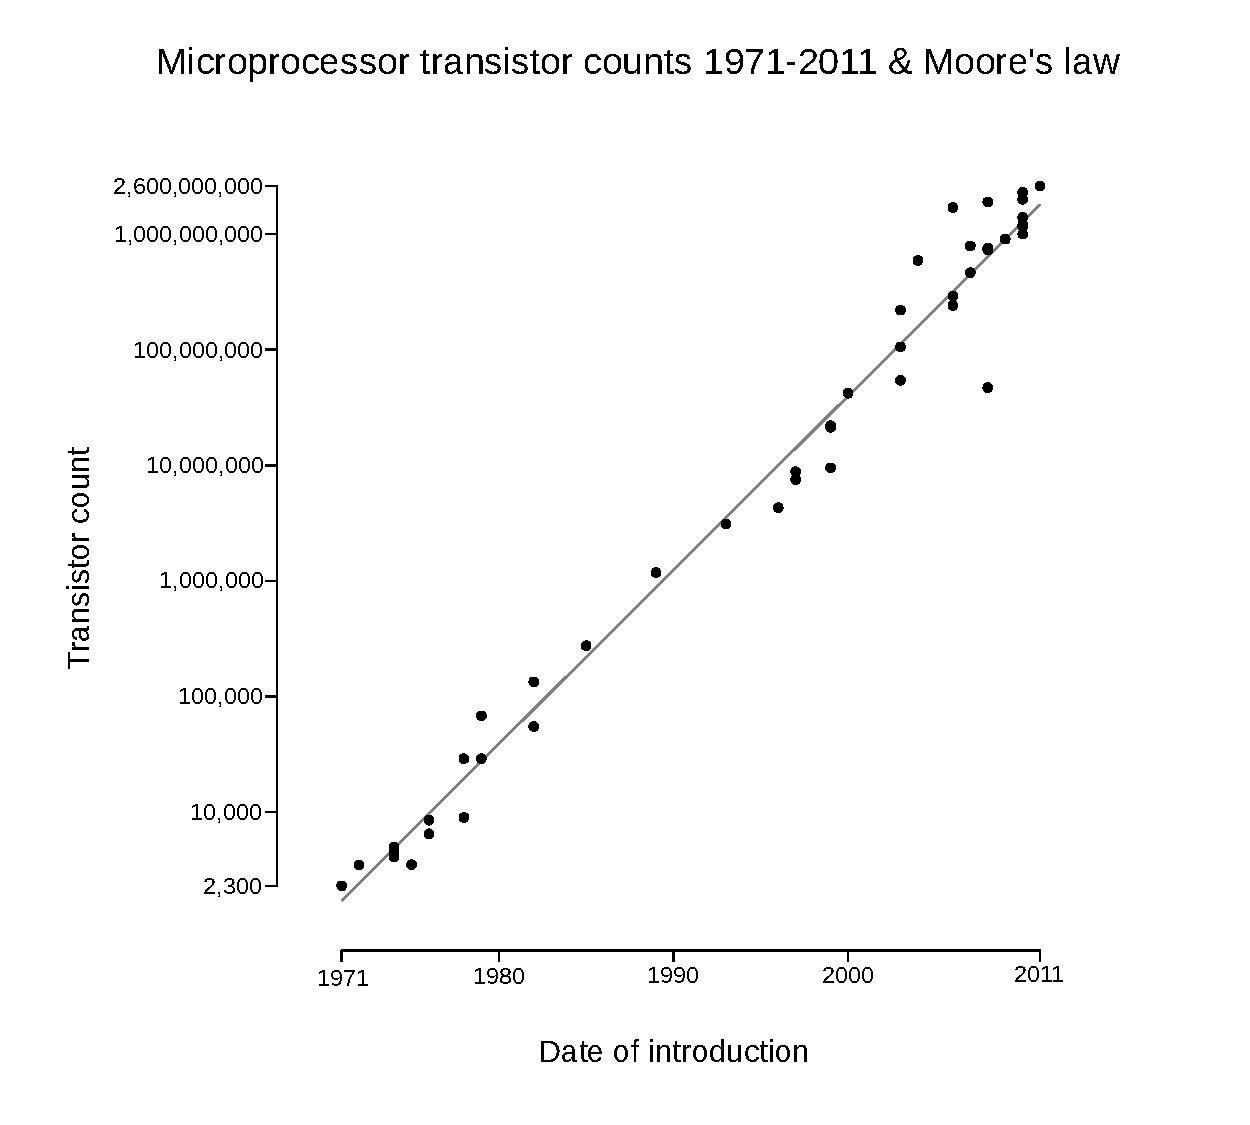
\includegraphics[scale=0.4]{pics/moore}
\end{figure}
\noindent
This is problematic, since there will be a time when the distance between the transistors will be entering the quantum regime (as the chip size remains constant) and classical physics breaks down as quantum effects begin to interfere in the functioning of electronic devices as they are made smaller and smaller. \\[0.2cm]
The solution for this was to change the paradigm. Instead of treating quantum effects as a interference, we started to develop quantum computers which uses quantum mechanics as an operating system to perform computations.\\[0.2cm] 
Note that, a classical computer \textit{can} simulates quantum mechanics, but not efficiently! Classical algorithms would take \textit{superpolynomial} or \textit{exponential} time to run a quantum computation.\\[0.2cm]
This concept of efficiency led to the strengthening of the Church-Turing thesis
\begin{center}
    ``Any algorithmic process can be \textit{efficiently} simulated by a universal Turing machine''
\end{center}
This is helpful since, if this thesis is true, then instead of analysing different models of computation for a given task, we can restrict ourselves to the Turing machine model for the computation of the task. \\[0.2cm]
A challenge to this statement came when \textit{randomised algorithms} were introduced. These algorithms used random numbers to perform a task. However, Turing machines were \textit{deterministic} and thus suggesting that efficiently soluble problems exist which cannot be efficiently solved on a deterministic Turing machine. One such algorithm is the \textit{Solovay-Strassen} test which is a primality test. 
\begin{algorithm}[Solovay-Strassen]\hspace*{0.1cm}
\begin{algorithmic}[1]
\Require $n$, a value to test for primality and $k$, a parameter that determines the accuracy of the test 
\Ensure composite if $n$ is composite and otherwise prime with some \textit{uncertainty}
\For{$n = 1, \dots, k$}
    \State choose $a$ randomly from $[2,n-1]$
    \State $x \gets \qty(\frac{a}{n})$ 
    \If{$x=0$ or $a^{(n-1)/2}\not\equiv x \ \qty(\mathrm{mod}\ n)$}
    \State \Return composite 
    \EndIf
    \EndFor\\
\Return probably prime
\end{algorithmic}
\end{algorithm}
The problem posed by probabilistic algorithms can be resolved by the modified Strong Church-Turing thesis,
\begin{center}
    ``Any algorithmic process can be simulated efficiently using a
probabilistic Turing machine''
\end{center}
This modification is kinda \textit{ad hoc} and leads us to think that someday some new kind of computation will be developed which will lead to some further modification in the thesis. Thus we need to find a  single model of computation which is guaranteed to simulate any other model of computation.\\[0.2cm]
On this note, David Deutsch tried to use physical laws to develop a computational model. He attempted to formalise a model which will simulate any arbitrary physical system. Since quantum mechanics makes the foundation of natural laws, the idea of a \textit{universal quantum computer} was established!\\[0.2cm]
In his 1981 paper \textit{Simulating Physics with Computer}, Feynman proposed the notion of a quantum computer. In a quantum computer, the algorithms also need to be quantum mechanical. \\[0.2cm]
In 1994, Peter Shor developed an algorithm that enables finding prime factors of a number. This problem is in general hard, since given a number, say, $2153415191$ we have to grind our minds to find out that it has two prime factors $64817$ and $33223$. However, the reverse problem is easy, given a number $p$ we can check whether it is a factor of $n$, just by simple division.\\[0.2cm]
The most efficient classical algorithm to factor large integers is the \textbf{general number field sieve} which has a sub-exponential time complexity, of the order of, $\exp\qty(\qty(\frac{64}{9})^{1/3}(\ln N)^{1/3}(\ln \ln N)^{2/3})$. However, as the number of digits increases, this takes a lot of time to factor. For about 400 digits, it takes $10^{10}$ years to factor, which is about the age of the Universe. On the other hand, on a quantum computer, using Shor's algorithm, it would take around three years to factorise a 400 digit number, which is way way better in time.
